\documentclass{beamer}

\usepackage{import}
\usepackage{xifthen}
\usepackage{pdfpages}
\usepackage{transparent}


% This file is a solution template for:

% - Talk at a conference/colloquium.
% - Talk length is about 20min.
% - Style is ornate.



% Copyright 2004 by Till Tantau <tantau@users.sourceforge.net>.
%
% In principle, this file can be redistributed and/or modified under
% the terms of the GNU Public License, version 2.
%
% However, this file is supposed to be a template to be modified
% for your own needs. For this reason, if you use this file as a
% template and not specifically distribute it as part of a another
% package/program, I grant the extra permission to freely copy and
% modify this file as you see fit and even to delete this copyright
% notice. 


\mode<presentation>
{
  \usetheme{Berlin}
  \setbeamercovered{transparent}
}


\usepackage[spanish,mexico]{babel}
\usepackage[utf8]{inputenc}
\usepackage{times}
\usepackage[T1]{fontenc}

\title{Plataforma Gough-Stewart}

\subtitle
{Reporte de medio término}

\author[]{E. Benavides \and I. Ayala \and N. González}


\institute[]
{
  Centro de Investigación y de Estudios Acanzados del IPN\\
  Robótica y Manufactura Avanzada
  }

\date[]{RyMA 2019}

\subject{Robotics}



% Delete this, if you do not want the table of contents to pop up at
% the beginning of each subsection:
\AtBeginSubsection[]
{
  \begin{frame}<beamer>{Outline}
    \tableofcontents[currentsection,currentsubsection]
  \end{frame}
}


% If you wish to uncover everything in a step-wise fashion, uncomment
% the following command: 

%\beamerdefaultoverlayspecification{<+->}



\begin{document}

{

\usebackgroundtemplate%
{%
%     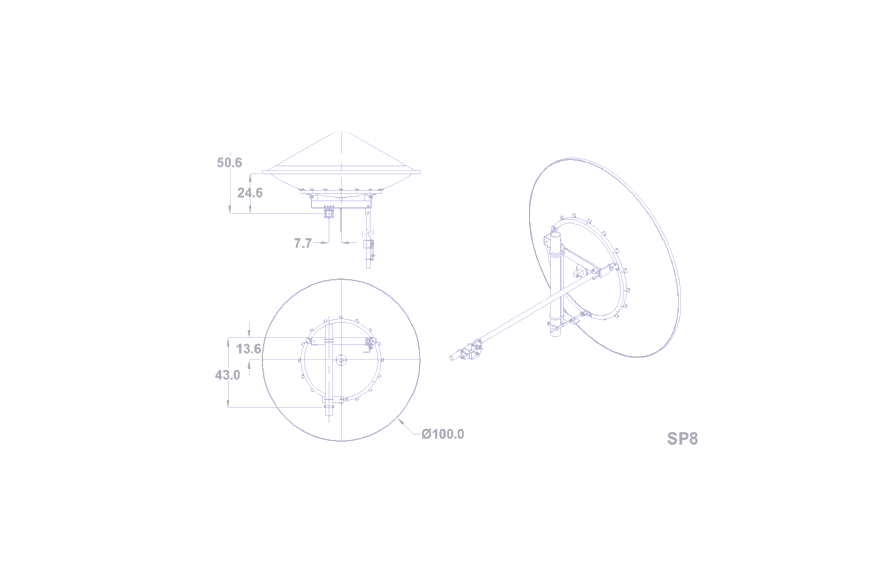
\includegraphics[width=\paperwidth,height=\paperheight]{antenna.png}%
}
\begin{frame}
  \titlepage
\end{frame}}

\begin{frame}{Contenido}
  \tableofcontents
\end{frame}



\section{Introducción}

\subsection{Nomenclatura}
\begin{frame}{Definiciones}
\begin{itemize}
 \item Masa del disco parabólico $m_{dp}$
 \item Centro de masa del disco parabólico $cm_{dp}$
 \item Punto de unión del pistón en la plataforma $a_i$
 \item Punto de unión del pistón en la base $b_i$
 \item Vector unitario del pistón $u_i$
 \item Velocidad lineal del pistón $v_p$
\end{itemize}

 
\end{frame}


\subsection{Motivación}

\begin{frame}{Uso de la plataforma Gough-Stewart}

  \begin{itemize}
    \item Movimiento preciso de objetos 
    \item Control preciso de la posición de antenas parabólicas
    \begin{itemize}
     \item Antena parabólica SP8-2.1 de la compañía \emph{radiowaves}
    \end{itemize}

  \end{itemize}
  
\end{frame}

{
\usebackgroundtemplate%
{%
}

\begin{frame}{Aplicación}
 \begin{figure}[h]
 \centering
 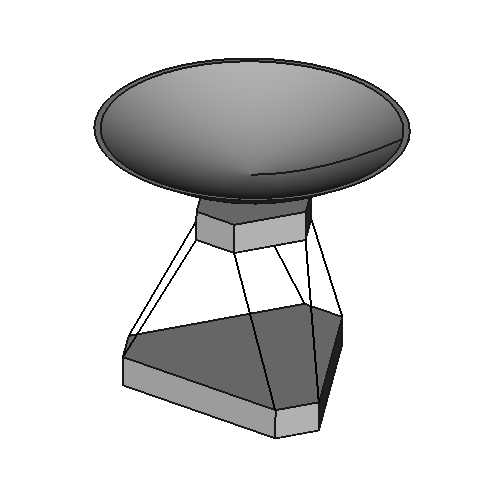
\includegraphics[scale=0.4]{../img/implementation.png}
 % implementation.png: 495x490 px, 96dpi, 13.10x12.96 cm, bb=0 0 371 367
 \caption{Aplicación de la plataforma Gough-Stewart.}
 \label{fig: antenna}
\end{figure}

\end{frame}
}

\section{Desarrollo}

\subsection{Cinemática}

{
\usebackgroundtemplate%
{%
}
\begin{frame}{Abstracción del modelo}{}
 \begin{center}
 \begin{figure}
 \import{../img/}{goughStewart.pdf_tex} 
 \caption{Abstracción de geometría.}
 \label{key: diagram}
 \end{figure}

 
 \end{center}

\end{frame}}

\begin{frame}{Relación de posiciones}

\begin{itemize}
 \item Se establece la relación de posición entre la base y la plataforma\\
 \begin{equation}
  p_i = d + Ra_i = b_i + l_i
  \label{eq: position}
 \end{equation}
 \item La ecuación \ref{eq: position} se expresa en función de la longitud $l_i$ de cada pistón
 \begin{equation}
  l_i = d + Ra_i - b_i
 \end{equation}
\end{itemize}

\end{frame}

\begin{frame}{Transformaciones homogéneas}
\begin{itemize}
 \item Definimos $R$ como la matriz de rotación extrínseca de la plataforma respecto a la base. \\
 \begin{equation}
R = R_zR_yR_x = R_{xyz}
\end{equation}
\end{itemize}
\end{frame}

\begin{frame}{Coordenadas generalizadas}
 \begin{itemize}
  \item Designamos $||l_i||$ como las coordenadas generalizadas $q_i$
  
  \begin{equation}\label{eq_coordgral}
q_i = ||l_i|| = \sqrt{l_i^Tl_i}
\end{equation}
  
 \end{itemize}

\end{frame}


\begin{frame}{Jacobiano inverso}
\begin{itemize}
 \item Considerando
 
 \begin{equation}
\dot{q}_i=J^{-1} \nu = A \begin{bmatrix}
v_p\\
\omega
\end{bmatrix} \Rightarrow A = J^{-1}
\end{equation}

\item Derivando la ecuación \ref{eq_coordgral} se obtiene

\begin{equation}
\dot{q}_i=\frac{1}{||l_i||}(\dot{d} + [\omega \times] Ra_i)\cdot(d + Ra_i -b_i) 
\end{equation}

\end{itemize}

 
\end{frame}

\begin{frame}{Jacobiano inverso}

\begin{itemize}
 \item Desarrollando
 \begin{equation}
\dot{q}_i = \frac{1}{||l_i||} \left( v_p  \cdot l_i + [(Ra_i)\times]l_i \cdot \omega \right )
\end{equation}
 \item Se obtiene
\begin{equation} 
\label{eq: inverse jacobian}
\dot{q}_i = \frac{1}{||l_i||} [l_i^T , [(Ra_i)\times]l_i^T] \begin{bmatrix}
v_p\\
\omega
\end{bmatrix}
\end{equation}
 
\end{itemize}



\end{frame}

\begin{frame}{Jacobiano}
 \begin{itemize}
  \item De la ecuación \ref{eq: inverse jacobian} se llega a 
  
  \begin{equation}\label{jac_A}
        A = J^{-1} = 
        \begin{bmatrix}
            \vec{u_i}^T, & [(Ra_i)\times]\vec{u_i}^T
        \end{bmatrix}
\end{equation}

\item Dado que $J = A ^{-1}$

\begin{equation}
J = \begin{bmatrix}
\vec{u_i}^T, & [(Ra_i)\times]\vec{u_i}^T
\end{bmatrix}^{-1}
\end{equation}
 \end{itemize}

\end{frame}

\subsection{Energía}
\begin{frame}{Energía cinética del sistema}

\begin{itemize}
 \item Obtenemos las velocidades del sistema
 \begin{equation}
\begin{bmatrix}
\vec{u_i}^T, & [(Ra_i)\times]\vec{u_i}^T
\end{bmatrix}^{-1} \dot{q} = \begin{bmatrix}
v_p\\
\omega
\end{bmatrix}
\end{equation}

\item Expresamos la energía cinética $K$ del sistema

\begin{equation}
 K = \frac{1}{2} ||v_{p}||^2 m_{dp}  + \frac{1}{2} \omega^T I \omega 
\end{equation}


\end{itemize}
\end{frame}

\begin{frame}{Energía Potencial}
 \begin{itemize}
  \item La energía potencial
  \begin{equation}
\begin{split}
P_{dp} = m_{dp}gh = [0\ 0\ m_{dp}g] \begin{bmatrix}
P_x\\
P_y\\
P_z\\
\end{bmatrix}\\
\\
P_z = d + R\begin{bmatrix}
0\\
0\\
cm_{dp}\\
\end{bmatrix}\\
\end{split}
\end{equation}
  
 \end{itemize}

\end{frame}


\section{Simulador}
\subsection{MATLAB}
\begin{frame}{GSP Toolbox}
 \begin{itemize}
  \item Simulador programado en MATLAB
  \item Interfaz gráfica
 \end{itemize}

\end{frame}

{
\usebackgroundtemplate%
{%
}
\begin{frame}{Interfaz gráfica}
 \begin{center}
  \begin{figure}[h]
 \centering
 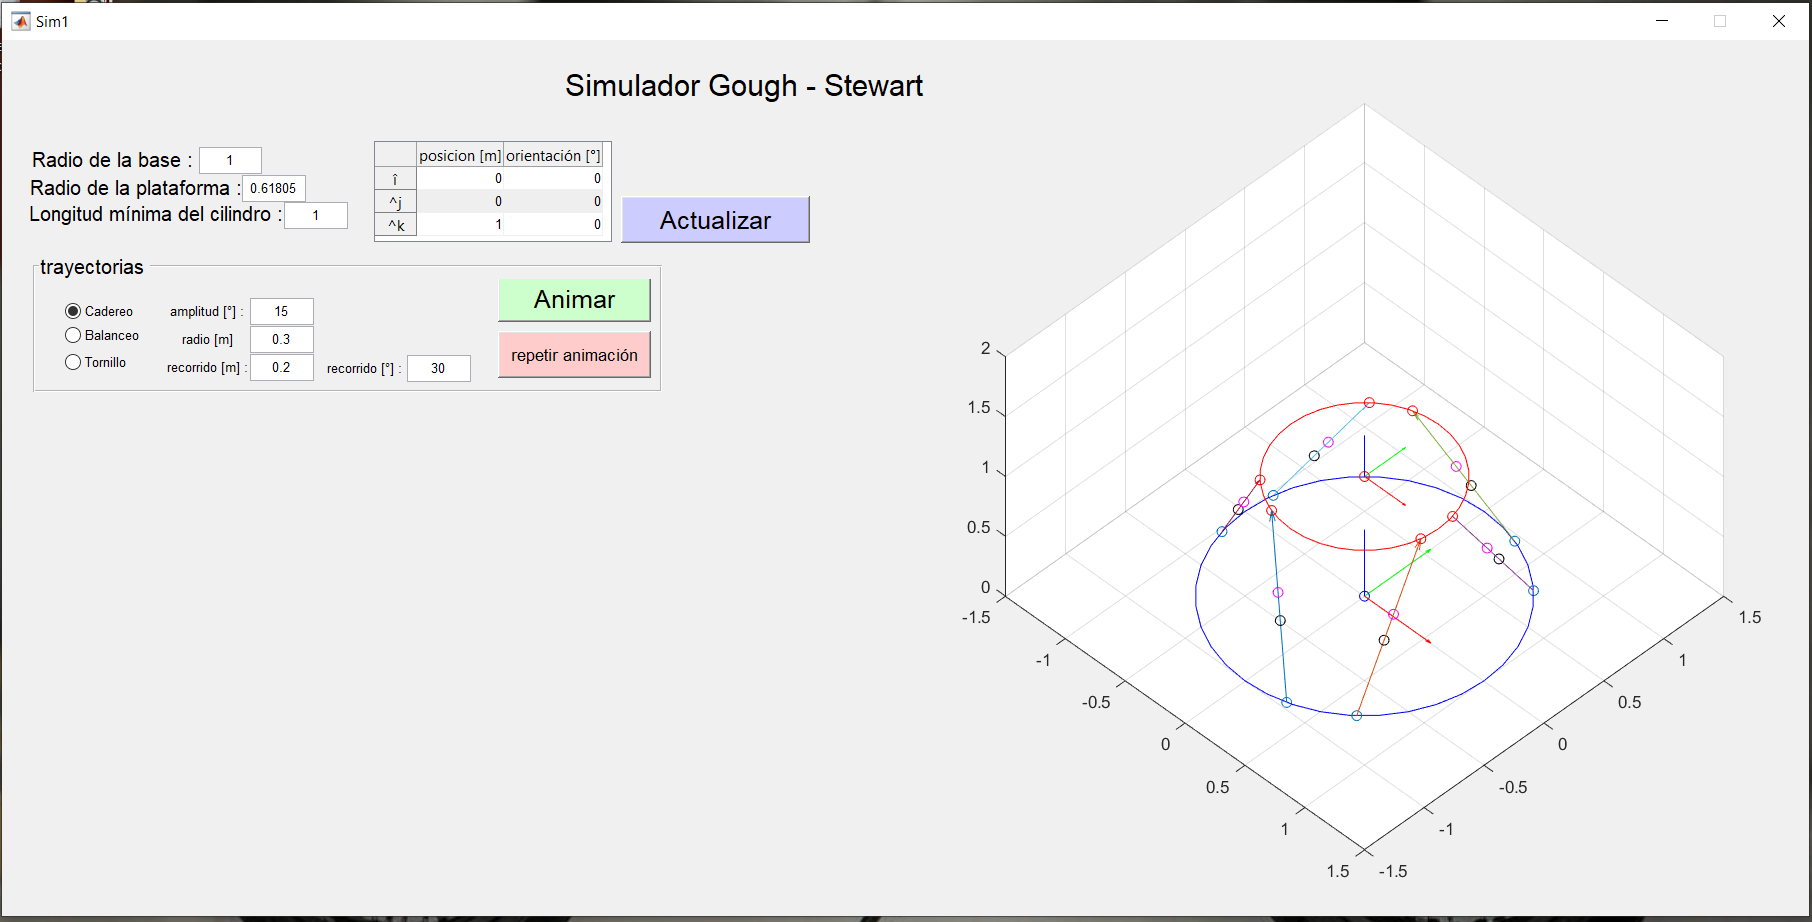
\includegraphics[scale=0.2]{../../04_Manual/img/principal.PNG}
 % principal.PNG: 1812x922 px, 120dpi, 38.36x19.52 cm, bb=0 0 1087 553
 \caption{Interfaz gráfica del simulador.}
 \label{fig: GUI}
\end{figure}

 \end{center}

\end{frame}}




\end{document}


